\section{Comparaisons}
\begin{figure}[H]
    \centering
    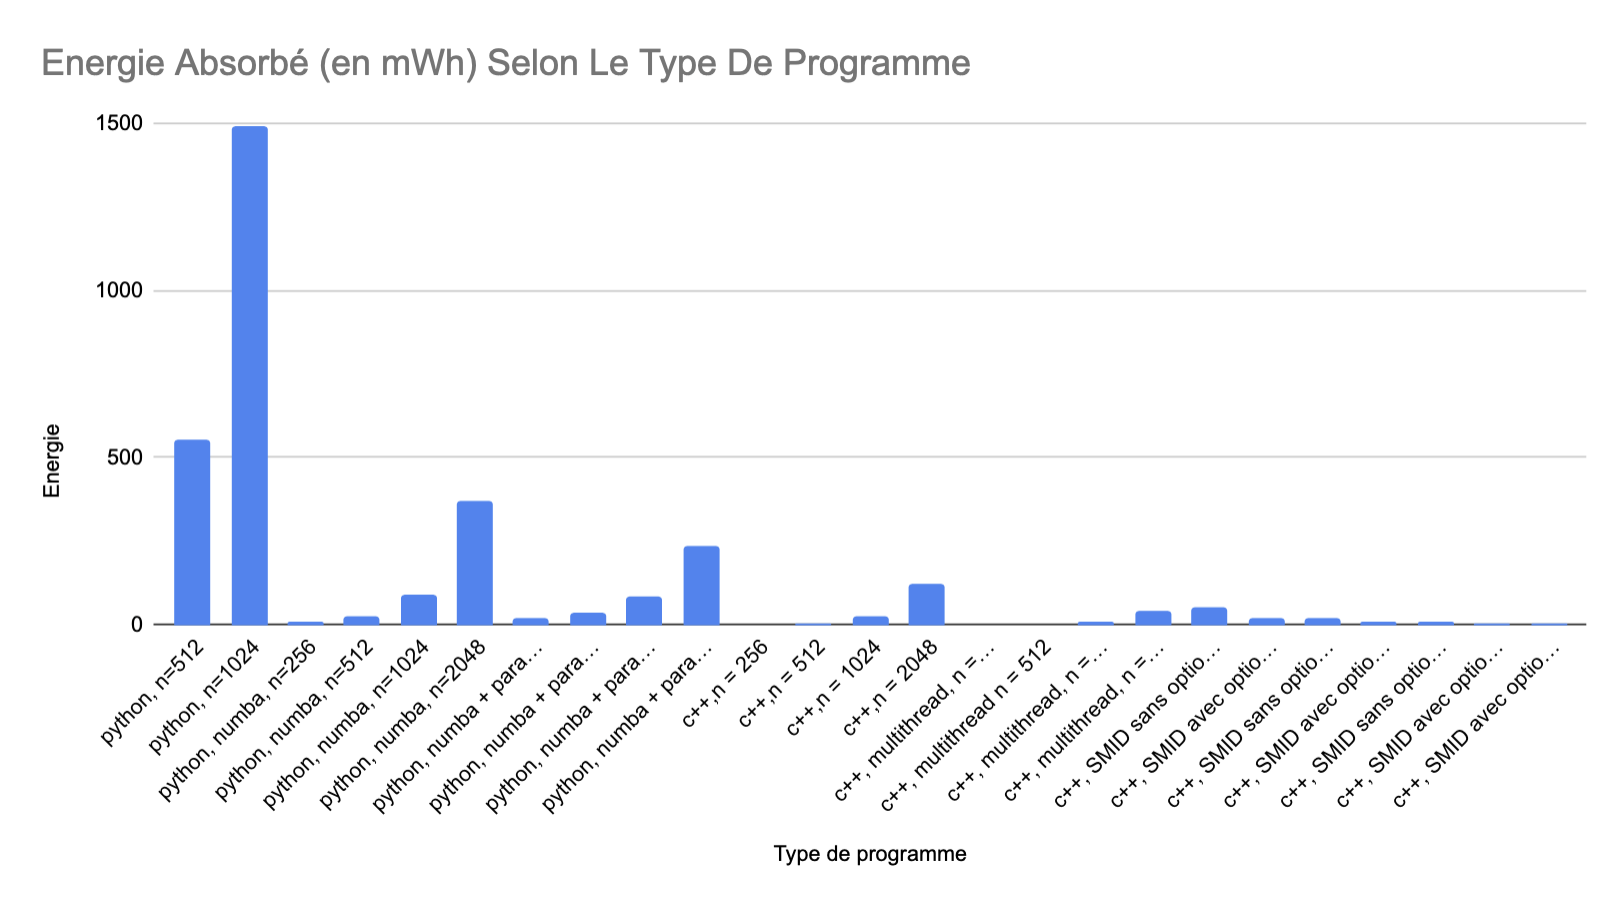
\includegraphics[width=0.85\textwidth]{images/graph1.png}
    \caption{Consommation énergétique selon les différentes versions}
\end{figure}

On observe assez nettement que les exécutions réalisées en Python consomment significativement plus d’énergie que les autres versions.  
Cependant, l’utilisation de \texttt{numba}, notamment en mode parallèle, permet de réduire considérablement cette consommation grâce à des temps d’exécution beaucoup plus courts.  
En ce qui concerne le langage C, il s’avère bien moins énergivore que Python. De plus, le recours au multithreading et au parallélisme contribue à diminuer encore davantage la consommation énergétique.
 


\begin{figure}[H]
    \centering
    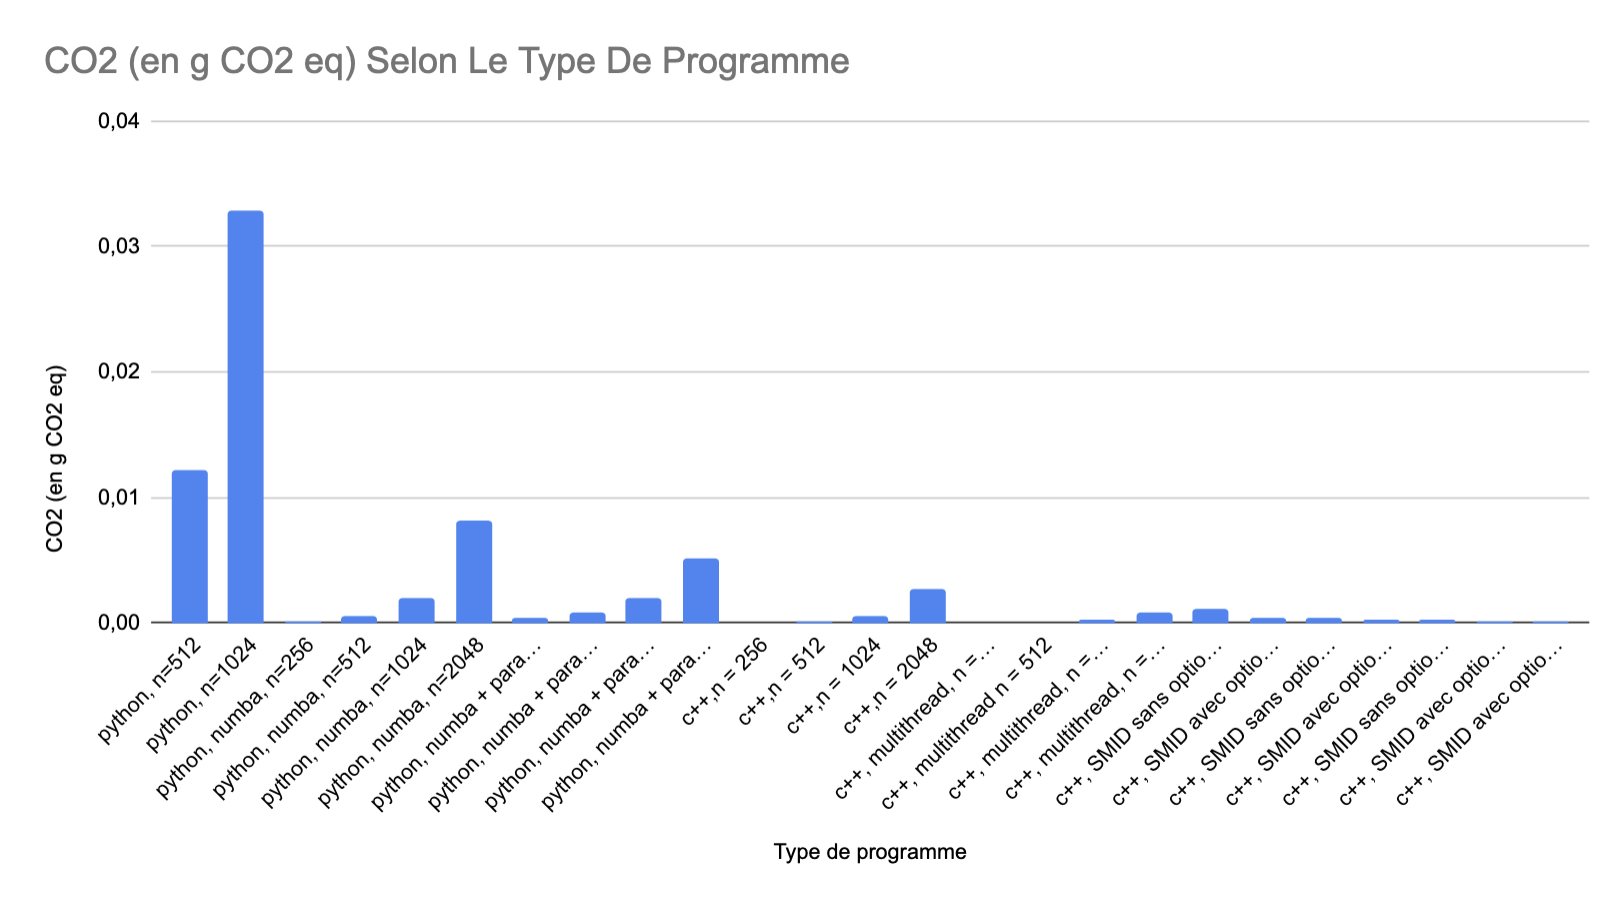
\includegraphics[width=0.85\textwidth]{images/graph2.png}
    \caption{Emission de CO2 selon les différentes versions}
\end{figure}

En ce qui concerne les émissions de CO2, on retrouve des tendances similaires à celles observées pour la consommation énergétique. Les programmes écrits en Python, en particulier sans optimisation, génèrent davantage d’émissions du fait de leur durée d’exécution plus longue.  
L’usage de \texttt{numba}, notamment en mode parallèle, permet de limiter ces émissions en réduisant le temps de calcul.  
Le langage C, de son côté, se révèle plus sobre en émissions de CO2, et les optimisations par multithreading ou parallélisme contribuent à minimiser encore davantage l’impact environnemental du programme.


\begin{figure}[H]
    \centering
    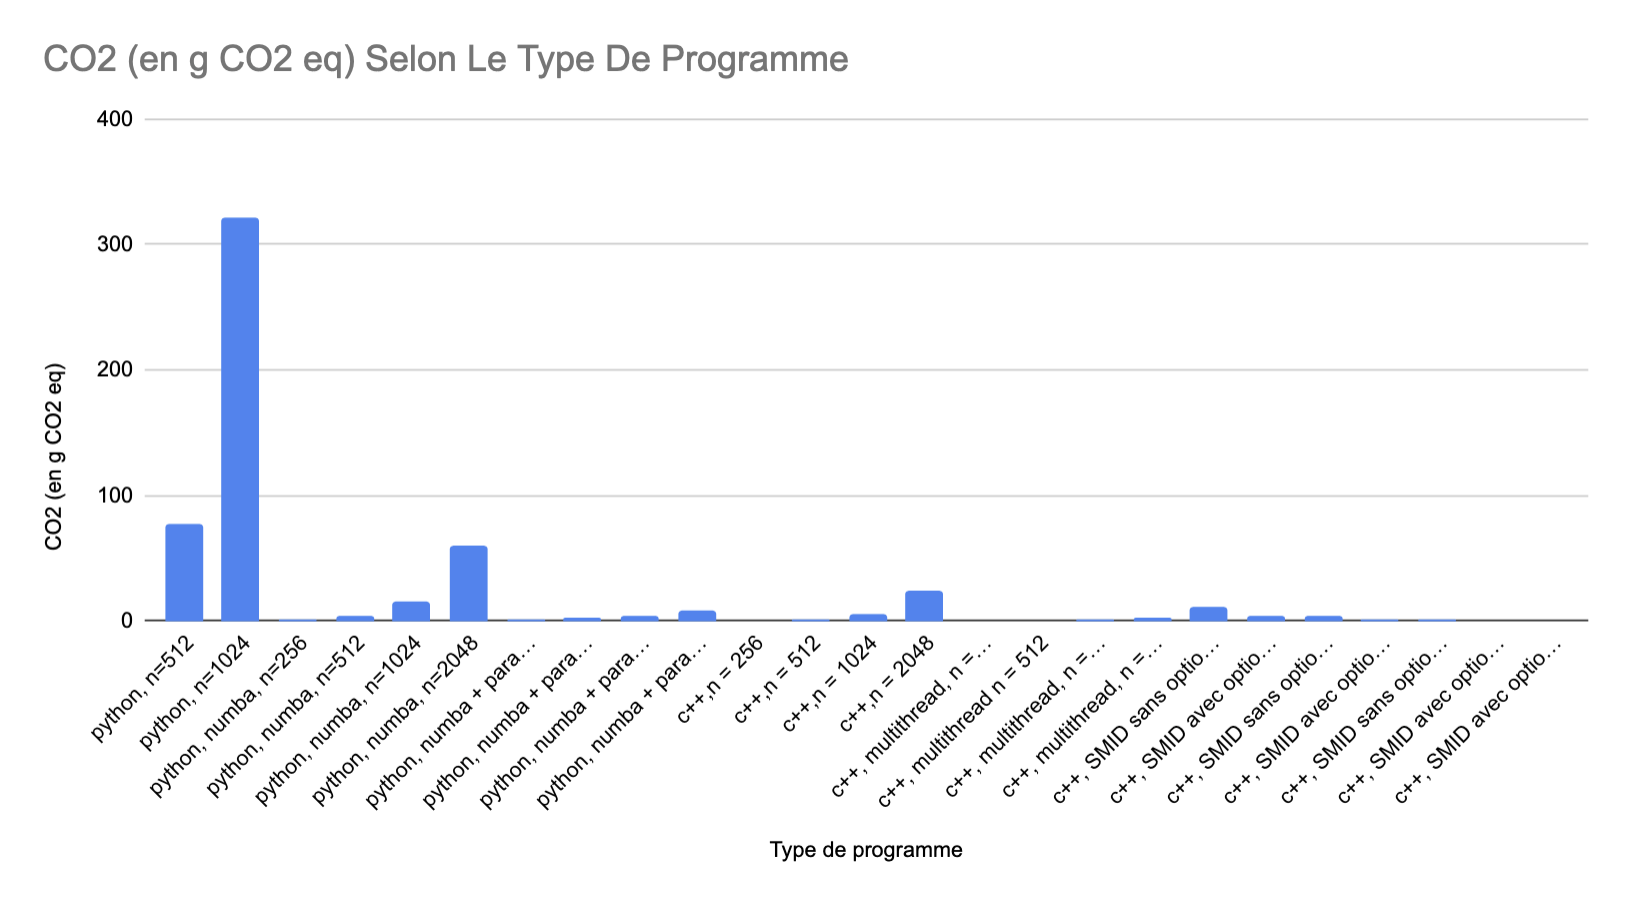
\includegraphics[width=0.85\textwidth]{images/graph3.png}
    \caption{Temps d'execution selon les différentes versions}
\end{figure}
Le temps d’exécution constitue un critère central dans cette étude, car il influe directement sur la consommation énergétique et les émissions de CO2.  
Les programmes écrits en Python, sans optimisation, présentent des temps d’exécution très élevés, en particulier lorsque la taille de l’image augmente. L’intégration de \texttt{numba} permet de diviser ces temps par un facteur important, et l'exécution en parallèle renforce encore ces gains.  
Les programmes compilés en C offrent naturellement de très bons temps d’exécution, souvent bien meilleurs que ceux de Python. L'utilisation du multithreading ou du parallélisme permet alors d’atteindre des performances encore plus optimales, avec des temps d’exécution particulièrement faibles.

Au terme de ce travail, nous avons pu comparer l’impact énergétique, les émissions de CO2 et les temps d’exécution de différents programmes réalisés en Python et en C.
L’étude met en évidence l’importance de l’optimisation du code, tant en termes de performances que d’impact environnemental.
Les programmes Python non optimisés se révèlent particulièrement coûteux en énergie et en temps. L’utilisation de \texttt{numba}, surtout avec exécution parallèle, améliore significativement les performances.
Le langage C, quant à lui, confirme sa réputation d’efficacité, avec une consommation énergétique plus faible et des temps d’exécution bien meilleurs, encore optimisables grâce au multithreading.
Ces résultats montrent qu’un choix judicieux du langage et des méthodes d’optimisation permet non seulement de gagner en rapidité, mais aussi de réduire l’empreinte carbone des applications informatiques.